\mysection{3}{Graph Importance}
\subsection{Importanza dei Nodi nei Grafi}

In molte applicazioni che coinvolgono grafi, come le reti sociali, i motori di ricerca, i sistemi di raccomandazione e le reti di trasporto, è fondamentale determinare quanto un nodo sia \textit{importante} o \textit{centrale} all'interno della struttura della rete. Esistono diversi approcci per quantificare tale importanza, e uno dei più efficaci è basato sul concetto di \textbf{passeggiata casuale} (\textit{random walk}) su un grafo.

In questa sezione, esploreremo le principali tecniche per valutare l'importanza dei nodi utilizzando strumenti probabilistici, concentrandoci in particolare su:
\begin{itemize}
    \item il concetto di \textbf{random walk} su grafi diretti e non diretti;
    \item la \textbf{probabilità di transizione} tra nodi, che rappresenta la probabilità che un cammino casuale si sposti da un nodo all'altro;
    \item le misure di importanza derivate da questi concetti, come il \textit{PageRank}.
\end{itemize}

Questi strumenti permettono di modellare dinamiche realistiche nei grafi e di identificare i nodi che, per posizione o connettività, svolgono un ruolo cruciale nella diffusione dell'informazione, nell'accessibilità o nel controllo della rete.

\subsection{Random Walk}
É una tecnica che consiste nel percorrere il grafo \textbf{casualmente}. Partendo da un nodo qualsiasi, cominciamo a scorrere il grafo (se diretto, nella direzione corretta) e ci fermiamo quando vogliamo, contando peró le ripetizioni di tutti i nodi (ovvero quante volte incontriamo ogni nodo nel nostro cammino). 

\subsubsection*{Transition Probability in a Graph}
Dato un nodo $N_i$, qual é la probabilitá che percorrendo K passi casuali si arrivi ad un nodo $N_j$? Chiamiamo questa misura \textbf{transition probability}. 
\\
Potremmo anche decidere di fare una pausa, fermarci per saltare ad un altro nodo: dovremo quindi aggiungere alla transition probability la \textbf{teleport probability}, ovvero la probabilitá di fare un salto. La somma delle due probabilitá deve andare a 1:
\[
P_{teleport} + P_{transition} = 1
\]
Normalmente la teleport probability viene indicata con $\alpha$ ed é un parametro del random walk.  

\newpage

\subsubsection*{Markov Model}

Un \textbf{Modello di Markov} per grafi è una rappresentazione matematica del movimento stocastico (random walk) su un grafo, in cui la probabilità di passare da un nodo ad un altro dipende unicamente dallo stato corrente e non dalla sequenza di stati precedenti. Tale proprietà è nota come \textit{Markov property}.

\paragraph{Definizione formale}

Sia $G = (V, E)$ un grafo orientato, dove:
\begin{itemize}
    \item $V = \{v_1, v_2, \ldots, v_n\}$ è l'insieme dei nodi (o stati),
    \item $E \subseteq V \times V$ è l'insieme degli archi (o transizioni).
\end{itemize}

Si definisce una \textbf{matrice di transizione} $P \in \mathbb{R}^{n \times n}$ tale che:
\[
P_{ij} = \mathbb{P}(X_{t+1} = v_j \mid X_t = v_i)
\]
cioè la probabilità di muoversi dal nodo $v_i$ al nodo $v_j$ in un singolo passo.

La matrice $P$ è \textbf{stocastica per righe} (o per colonne, a seconda della convenzione): ogni riga (in questo caso) deve sommare a 1:
\[
\sum_{j=1}^n P_{ij} = 1, \quad \forall i \in \{1, \ldots, n\}
\]

\paragraph{Evoluzione temporale}

Dato un vettore di distribuzione iniziale $\pi^{(0)} \in \mathbb{R}^n$, che rappresenta la distribuzione di probabilità iniziale sui nodi, l'evoluzione del sistema è data da:
\[
\pi^{(t+1)} = \pi^{(t)} P
\]
dove $\pi^{(t)}$ rappresenta la distribuzione di probabilità sui nodi al tempo $t$.

\paragraph{Teleportation e PageRank}

In molte applicazioni reali (ad esempio nel \textit{PageRank} di Google), si introduce una probabilità di \textbf{teleportation} $\alpha \in [0,1]$ per garantire che il modello sia ergodico (cioè che esista una distribuzione stazionaria unica).

La matrice di transizione diventa:
\[
P' = \alpha P + (1 - \alpha) \cdot \frac{1}{n} \mathbf{1} \mathbf{1}^T
\]
dove:
\begin{itemize}
    \item $\alpha$ è il parametro di damping (solitamente $\alpha \approx 0.85$),
    \item $\frac{1}{n} \mathbf{1} \mathbf{1}^T$ è la matrice di teleportation, che assegna probabilità uniforme a tutti i nodi.
\end{itemize}

\paragraph{Distribuzione stazionaria}

Una distribuzione $\pi^*$ è detta \textbf{stazionaria} se:
\[
\pi^* = \pi^* P
\]
cioè, se applicando la matrice di transizione, la distribuzione resta invariata. In modelli ergodici, esiste una distribuzione stazionaria unica che rappresenta il comportamento a lungo termine del processo di Markov.
\\
\newpage
Data la matrice di transizione T e considerando la teleport probability $\alpha$=0, dato il vettore iniziale $v$ di delle probabilitá di ogni nodo: uno step dal tempo $t_i$ al tempo $t_{i+1}$ corrisponde alla moltiplicazione $T^T\times v_i$ dove $T^T$ é la matrice trasposta e $v$ é normalizzato sulle colonne:
\\
\begin{figure}[th]
    \centering
    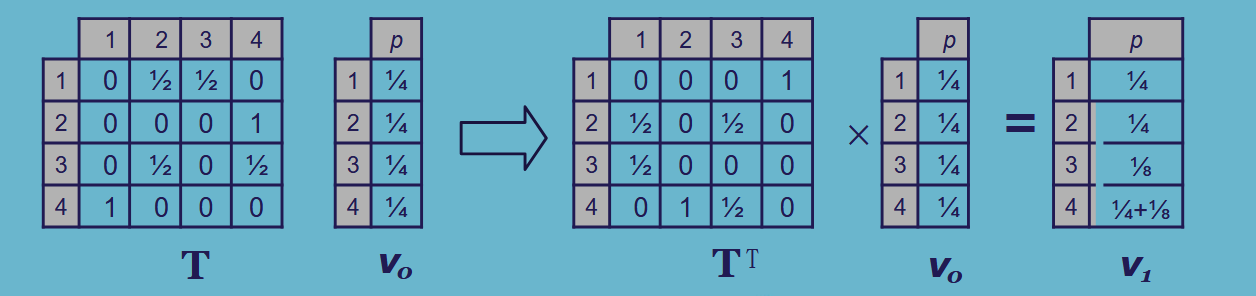
\includegraphics[scale=0.3]{GraphImportance//img/markov.png}
\end{figure}
\\
Considerando invece $\alpha \neq 0$, e ripetendo lo stesso ragionamento, consideriamo uno step temporale dal tempo $t_i$ al tempo $t_{i+1}$ come la moltiplicazione:
\\
\[
(1-\alpha)T^T\times v_i + \alpha \times v_0
\]
\begin{figure}[th]
    \centering
    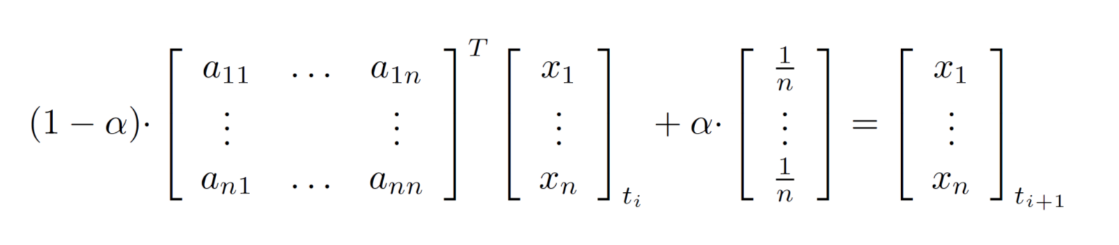
\includegraphics[scale=0.4]{GraphImportance//img/poweriteration.png}
\end{figure}
\\
E ci riferiamo a questo processo con il nome di \textbf{Power Iteration}. 
\newpage
\subsection{Co-Citation and Bibliographic Coupling}
Co-citation é uno degli ambiti dove si puó vedere l'applicazione del concetto di grafo. Indica la tecnica con cui si collegano ("linkano") due documenti. Quando un paper cita un altro, essi hanno una relazione, che puó essere studiata in \textbf{citation analysis}. Il grafo che connette piú documenti tra loro é un grafo diretto, aciclico: 
\\
\begin{figure}[th]
    \centering
    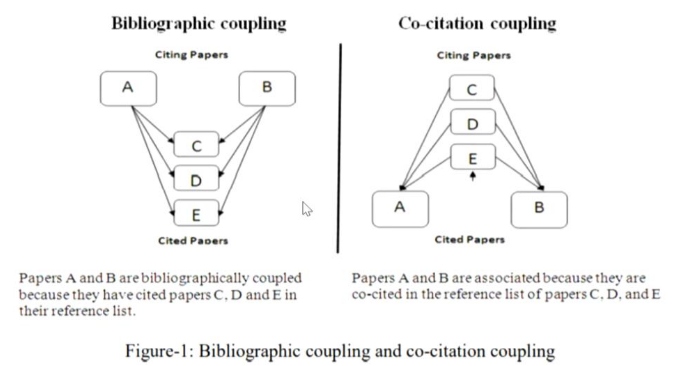
\includegraphics[scale=0.5]{GraphImportance//img/DAG.png}
\end{figure}
\\
In un \textbf{citation network} ogni nodo corrisponde ad un documento e gli archi sono le connessioni (citazioni). É quindi possibile dedurre:
\begin{itemize}
    \item se il nodo $A$ e il nodo $B$ sono connessi, e il nodo $A$ e il nodo $C$ sono connessi, é \textbf{probabile} che il nodo $B$ e il nodo $C$ siano connessi
    \item piú connessioni hanno in comune due nodi, piú quei nodi saranno simili, piú sará forte la loro \textbf{relazione}
\end{itemize}
\paragraph{Esempio} Costruiamo la matrice di adiacenza per un caso generale di co-citation. Come in un grafo non pesato indichiamo con 1 se é presente un arco, 0 se non é presente e chiamiamo la matrice $L_{ij}$. 
\\
Possiamo definire \textbf{Co-Citation}:
\[
C_{ij} = \sum_{k=1}^{n}L_{ki}L_{kj}
\]
come una misura di \textbf{similarity} basata sul numero di papers che co-citano $i$ e $j$. Si puó inoltre generare una matrice $\mathbb{C}$ quadrata sulla base di $C_{ij}$ chiamata \textbf{co-citation matrix} che indica sulla diagonale principale quante volte un articolo é stato citato dagli altri. 
\[
C_{ij} = L^T \times L
\]
\\
\begin{figure}[th]
    \centering
    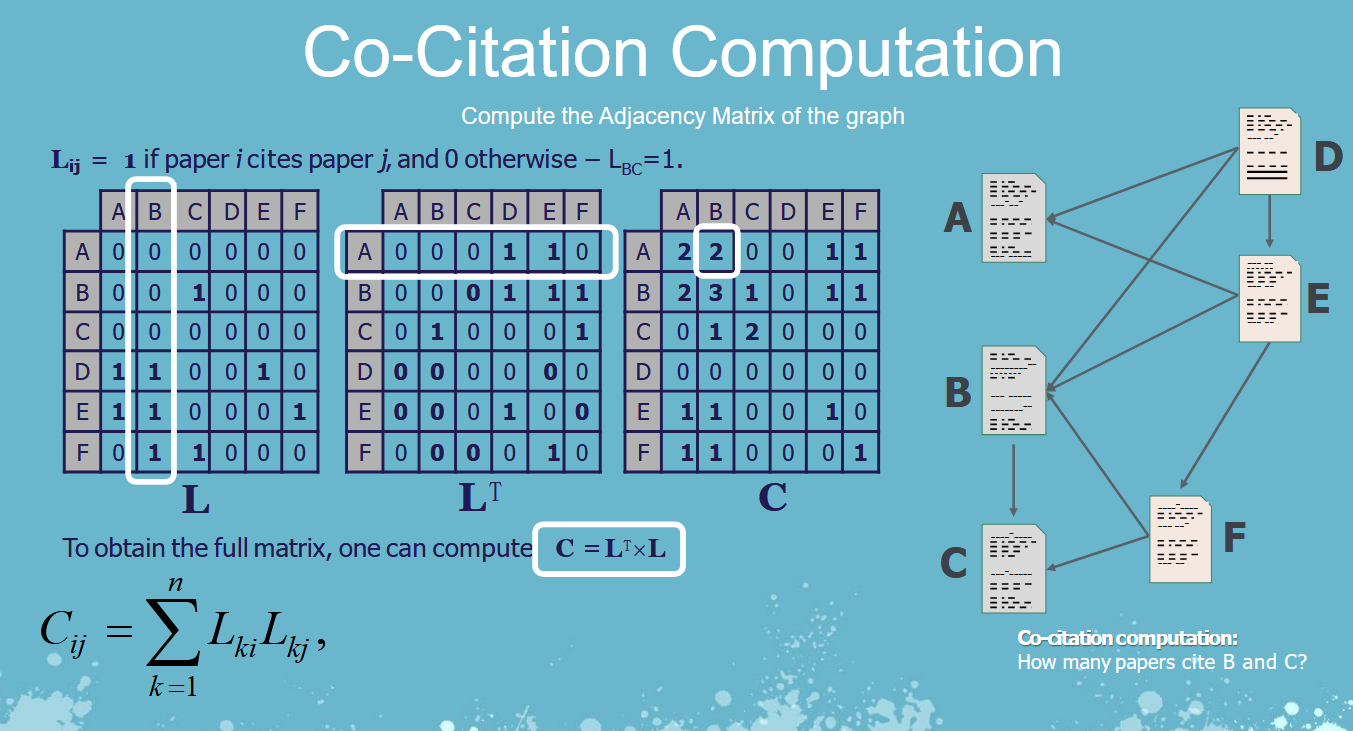
\includegraphics[scale=0.2]{GraphImportance//img/cocitationmatrix.png}
\end{figure}
\newpage
\subsubsection*{Bibliographic Coupling}
Si definisce in questo modo il caso in cui due diversi papers si riferiscano allo stesso paper nella loro bibliografia. Questo spesso indica che i due lavori siano in qualche modo correlati. 
\\
\textbf{Bibliographic Coupling} é simile a co-citation. Utilizziamo sempre una matrice e la chiamiamo $B_{ij}$ definita come:
\[
B_{ij} = \sum_{k=1}^{n} L_{ik} L_{jk}
\]
Che rappresenti il numero di papers che sono citati sia da $i$ che da $j$. Il termine $B_{ii}$ é il numero di references che ha il documento $i$. Questa matrice viene chiamata \textbf{bibliographic coupling matrix} e si puó ottenere in maniera analoga a come viene ricavata la co-citation matrix:
\[
B_{ij} = L \times L^T
\]
\begin{figure}[th]
    \centering
    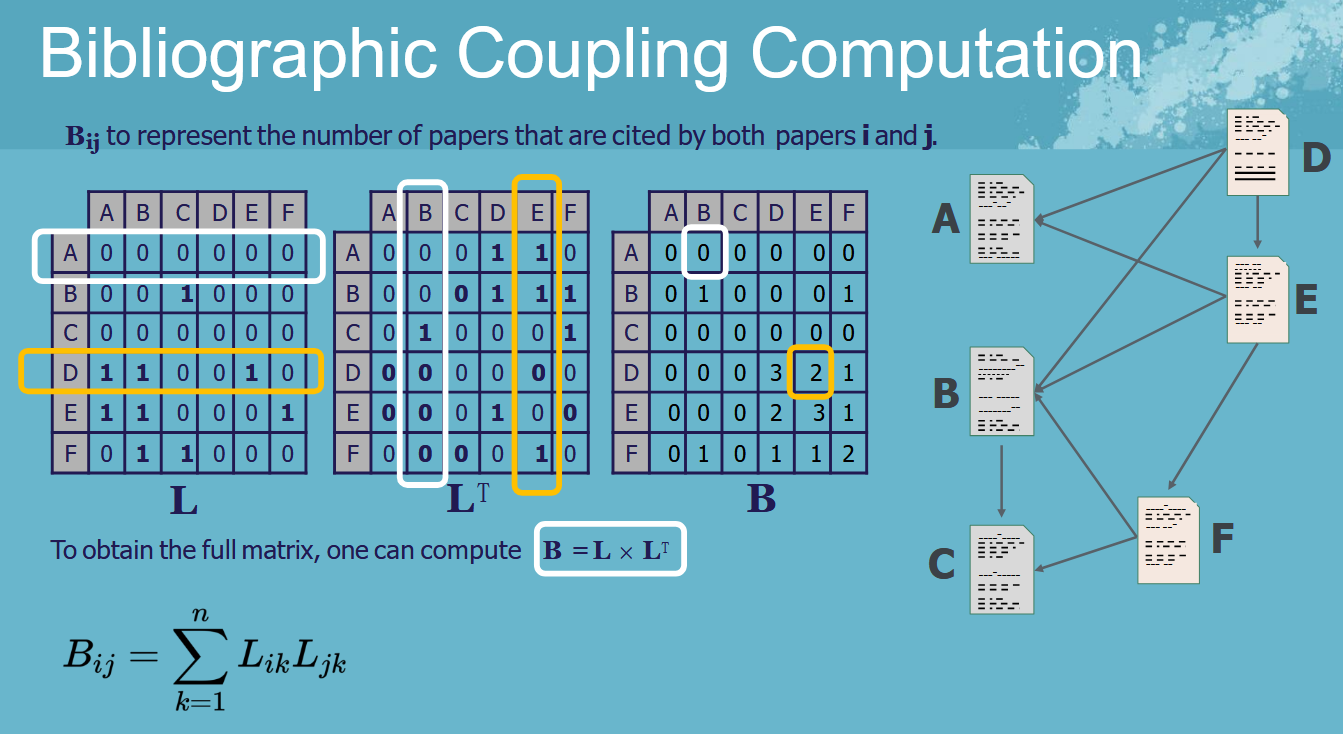
\includegraphics[scale=0.2]{GraphImportance//img/bibliocoupling.png}
\end{figure}
\\
La co-citazione tra articoli scientifici può essere utilizzata per molteplici finalità nel contesto dell'analisi della letteratura accademica. Può aiutare a \textbf{identificare ricerche correlate}, ovvero trovare articoli che esplorano tematiche o domande di ricerca simili. Inoltre, consente di \textbf{mappare i campi di ricerca}, visualizzando la struttura di un dominio scientifico e osservando come si connettono tra loro i diversi sottocampi. Può anche essere impiegata per \textbf{tracciare l'evoluzione scientifica}, studiando come si formano, evolvono o cambiano le comunità di ricerca e come si trasformano concetti, teorie o metodologie. Questo approccio permette di \textbf{trovare potenziali collaboratori}, identificando ricercatori che lavorano su problemi affini e aprendo opportunità di collaborazione. Inoltre, contribuisce a \textbf{migliorare la scoperta della letteratura}, rivelando articoli fondamentali che arricchiscono il processo di revisione con intuizioni più ampie e approfondite. È utile per \textbf{identificare comunità di ricerca}, portando alla luce cluster di lavori connessi, e per \textbf{mappare l'influenza scientifica}, scoprendo i contributi fondativi di un campo. Infine, consente di \textbf{costruire reti di citazioni}, visualizzando la struttura di un'area di studio e identificando gruppi densi di articoli correlati.

\subsection{Hypertext Induced Topic Search (HITS)}
\textbf{HITS} é un algoritmo per link analysis creato nel 1999 da Jon Kleinberg come metodo alternativo al PageRank per il ranking di pagine web. L'algoritmo introduce 2 aspetti fondamentali:
\begin{itemize}
    \item \textbf{Authority and Hub Scores}: HITS assegna ad ogni page due score, \textbf{authority score} e \textbf{hub score}. Il primo misura il valore della page in generale, il secondo misura il tipo di link che ha con le altre pagine
    \item \textbf{Mutual Reinforcement Relationship}: L'intuizione centrale dell'algoritmo HITS è il rafforzamento reciproco tra hub e autorità: alta autorità sono pagine che ricevono link da molte hub buone, buone hub sono pagine che puntano a molte autorità forti
\end{itemize}
HITS funziona sulla base di una query. L'utente immette una query di ricerca e HITS prima cerca con un motore, poi produce due liste: una per l'authority e una per l'hub. 
\\
Cosa sono effettivamente una pagina authority e una hub? Indichiamo con \textbf{hub} una pagina che ha tanti \textbf{out-links}, ovvero che é una pagina usata come organizer che linka a molte authorities, mentre un'\textbf{authority} é una pagina che ha molti \textbf{in-links} ovvero molte altre pagine linkano ad essa (discorso che non c'entra assolutamente nulla con i paper/documenti usati nel co-citation o bibliographic coupling).
\\
La relazione principale che intercorre tra i due dev'essere:
\begin{itemize}
    \item una buona authorities deve essere puntata da tante buone hub
    \item una buona hub deve puntare a tante buone authorities
\end{itemize}
Attenzione, ogni nodo ha due score quindi é ripetuto due volte in memoria (costo elevato). Procediamo iterativamente: 
\begin{enumerate}
    \item al tempo $t_0$ abbiamo due score per ogni nodo assegnato (generico, $\frac{1}{\sqrt{N}}$)
    \item al tempo $t_1$ accumuliamo gli score di ogni authority da ogni hub e viceversa
\end{enumerate}
Ripetendo questo processo ad ogni step, aggiornando ogni volta entrambi gli score.
\paragraph{Convergenza} Nel contesto dell’algoritmo HITS (Hyperlink-Induced Topic Search), dire che converge a un punto stabile significa che, dopo un certo numero di iterazioni, i punteggi di hub e di autorità assegnati a ciascuna pagina non cambiano più in modo significativo: raggiungono un valore stabile (o oscillano attorno a un valore molto vicino).
\\
\textbf{Perché succede?}
\\
HITS funziona aggiornando i punteggi delle pagine in modo iterativo:
\begin{itemize}
    \item Punteggio di autorità di una pagina = somma dei punteggi di hub delle pagine che la linkano.
    \item Punteggio di hub di una pagina = somma dei punteggi di autorità delle pagine a cui essa punta.
\end{itemize}
Dopo ogni aggiornamento, si normalizzano i punteggi (per evitare che crescano all’infinito) e si ripete il processo.
\\
Questo processo è simile a moltiplicare ripetutamente un vettore per una matrice, e sotto certe condizioni (come la connettività del grafo), questa sequenza di aggiornamenti converge all’autovettore principale della matrice corrispondente. Alla fine, i punteggi smettono di cambiare in modo rilevante: si dice che l’algoritmo é convergente ad un punto.
In pratica:
\begin{itemize}
    \item Dopo poche iterazioni (tipicamente meno di 100), i punteggi si stabilizzano.
    \item I valori stabili rappresentano quanto una pagina è un buon hub o una buona autorità nel contesto del grafo di collegamenti.
\end{itemize}

\paragraph{Esercizio} Calcola hub score e authority score del grafo seguente.
\\
\begin{figure}[th]
    \centering
    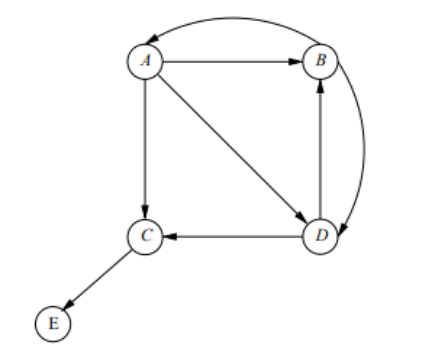
\includegraphics[scale=0.5]{GraphImportance//img/exercise.png}
\end{figure}
\\ 
Facciamo le giuste assunzioni per risolvere correttamente l'esercizio: 
\begin{itemize}
    \item N web pages (numero di nodi nel grafo, = 5)
    \item vettori \textbf{a} = ($a_1, ..., a_n$) authority score e \textbf{h} = ($h_1, ..., h_n$) hub score
    \item $\mathbb{A}$ adjacency matrix (matrice di adiacenza chiamata link matrix of the web) $N\times N$, grafo non pesato quindi sulle righe e colonne ha 1 se il link c'é, 0 se il link non c'é
\end{itemize}
Attenzione, essendo che:
\[
\textbf{h}_i = \sum_{i \rightarrow j} a_j
\]
Che vorrebbe dire che hub score della pagina $i$ é la somma dei punteggi di authority delle pagine a cui essa punta, ma quindi riscrivendolo usando $\mathbb{A}$:
\[
\textbf{h}_i = \sum_{i \rightarrow j} a_j = \sum_{j=1}^N \mathbb{A}_{ij} a_j = \mathbb{A} \cdot a
\]
Discorso uguale identico per l'authority score, ovviamente invertito: 
\[
\textbf{a}_i = \sum_{j \rightarrow i} h_j
\]
Perché per definizione l'authority score sarebbe la somma dello score degli hub che puntano a questa authority:
\[
\textbf{a}_i = \sum_{j \rightarrow i} h_j = \sum_{j=1}^N \mathbb{A}_{ji} h_j = \mathbb{A}^T \cdot h
\]
Quindi alla fine otteniamo che:
\\
\begin{figure}[th]
    \centering
    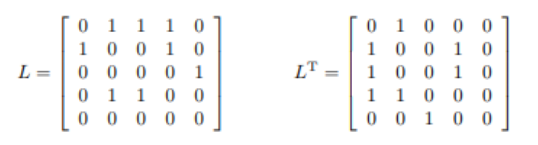
\includegraphics[scale=0.5]{GraphImportance//img/soluzione.png}
\end{figure}
\\
Matrice dei link del web: partendo da uno score $a,h=\frac{1}{\sqrt{N}}=\frac{1}{\sqrt{5}}$ si puó calcolare lo score dello step successivo, fino ad arrivare a:
\\
\begin{figure}[th]
    \centering
    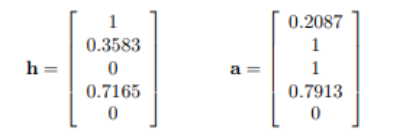
\includegraphics[scale=0.5]{GraphImportance//img/ah.png}
\end{figure}
\\

\newpage

\subsection{PageRank}
\textbf{PageRank} é un algoritmo che misura l'importanza dei nodi di un grafo dal tipo di struttura che li collega. Creato originariamente dai fondatori di Google Larry Page e Sergey Brin nel 1996-1997 a Stanford, ha rivoluzionato il mondo del web con una categorizzazione accurata delle pagine. 
\paragraph{Basic concept} Una pagina é importante se riceve link da altre pagine importanti. Questo crea una definizione \textbf{ricorsiva} dove l'importanza di una pagina viene definita da quanto sono importanti le pagine che puntano ad essa.

\paragraph{Modello matematico} Usa una struttura a grafo dove le pagine sono i nodi, i link tra le pagine sono archi e l'\textbf{importanza} di ogni pagina é distribuita su questi links.
\\
Il link dalla pagina $i$ alla pagina $j$ é un \textbf{voto} da $i$ a $j$; i voti da pagine con tanti voti \textbf{contano di piú}. In altre parole, ogni voto di ogni pagina é \textbf{proporzionale} all'importanza della pagina che lo emette. É quindi importante definire un \textbf{rank}:
\[
\textbf{r}_j = \sum_{i \rightarrow j} \frac{\textbf{r}_i}{d_i}
\]
Dove $d_i$ é \textbf{out-degree} del nodo $i$ ovvero il numero di archi uscenti dall'i-esimo nodo. Questo valore al denominatore serve a diluire il rank di quella pagina. 

\paragraph{Diluizione} Il valore di out-degree serve per distribuire equamente il pagerank della pagina $i$ tra tutte le pagine a cui si collega. Questo significa che se $\textbf{r}_i$ é 1, e la pagina $i$ é connessa ad altre 4, ad ognuna di esse arriverá $\frac{1}{4}$.  
\\
\textbf{Quindi out-degree diminuisce il valore di di rank della pagina $i$?} No. Lo diluisce tra le i suoi collegamenti, ma se la pagina $i$ ha un rank molto alto (dato dai rank delle pagine collegate a lei (in input) il valore $d_i$ non cambierá di molto il suo rank. Serve solo a far capire che se avesse un solo link, darebbe a quel nodo 1, mentre avendone 4 lo distribuisce.

\paragraph{Matrix Formulation} Definiamo una matrice stocastica sulle colonne (somma dei valori sulle colonne 1) $M_{ij}$, i cui valori sono 0 se due nodi non sono connessi, $\frac{1}{d_i}$ se i nodi sono connessi e definiamo inoltre un rank vector $r$ che ha un valore per ogni pagina (somma di tutti i suoi valori =1). L'\textbf{equazione del flusso} puó essere scritta in questo modo:
\[
r = M \cdot r
\]
Applicando il principio della \textbf{power iteration} all'equazione del flusso:
\[
r^{t+1}= M \cdot r^t
\]
Che si deve fermare quando:
\[
|r^{t+1} - r^t| > \varepsilon
\]
Questo modello é equivalente ad un random ralk con nessun teleport, quindi $\alpha =0$. Il risultato é una \textbf{distribuzione stazionaria}: il ranking finale delle pagine deriva dalla distribuzione stazionaria della catena di Markov che modella il comportamento di un utente che naviga il web seguendo solo i link. La distribuzione stazionaria é $r$, mentre la matrice di transizione é $M$ (tornando alla pagina 22 é possibile notare l'analogia con la definizione di distribuzione stazionaria).
\newpage
\paragraph{Stationary distribution} Data una matrice di transizione, e seguendo la power iteration, arrivo sempre ad una fine dei calcoli?
\\
La risposta é \textbf{dipende}. Per grafi che soddisfano determinate condizioni eventualmente la raggiungono ed é unica; inoltre é indipendente dalla distribuzione di probabilitá iniziale al tempo 0. Esistono convergenze problematiche:
\begin{itemize}
    \item \textbf{Dead-end}: nodo che non ha out-links, il random surfer si bloccherá lí facendo perdere informazione al next step (rimane fermo)
    \item \textbf{Spider Trap}: nodo con un ciclo ma senza uscita. Un loop, il random walk continuerá a camminare senza mai raggiungere la stabilitá
\end{itemize}
Per avere una convergenza e risultare una distribuzione stazionaria, é quindi necessario:
\begin{itemize}
    \item la matrice di transizione é stocastica sulle colonne,
    \item la matrice é \textbf{irriducibile}: il grafo é fortemente connesso, andata e ritorno per ogni coppia di nodi,
    \item la matrice é \textbf{aperiodica}: é possibile tornare ad ogni nodo con un numero finito di passi
\end{itemize}
Come posso quindi far sí che il modello segua le condizioni di Markov? Aggiungendo un parametro che mi colleghi tra loro tutti nodi: \textbf{damping factor}, o comunemente chiamato teleport, é la soluzione adottata da Google. Ad ogni step, si puó seguire un random link oppure saltare in un altro casuale evitando cosí spidertraps e deadends. L'equazione del PageRank risulta:
\[
r_j = \sum_{i \rightarrow j} \beta \frac{r_i}{d_i} + (1-\beta)\frac{1}{N}
\]
$\beta$ é il damping factor e 1-$\beta$ é la probabilitá di saltare ad un'altra pagina. La formulazione di Markov assume che non ci siano dead-ends: per funzionare, basta fare sí che se una colonna ha solo 0, si imposti un valore $\frac{1}{N}$. Riformulando:
\[
r = \mathbb{A} \cdot r
\]
dove
\[
\mathbb{A}_{ij} = \beta M_{ji} + \frac{1 - \beta}{N}
\]
Quindi:
\[
r_j=\sum_{i=1}^N \mathbb{A}_{ij}r_i = \sum_{i=1}^N [\beta M_{ji} + \frac{1 - \beta}{N}] \cdot r_i
\]
\[
r_j = \sum_{i=1}^N \beta M_{ji} \cdot r_i + \sum_{i=1}^N\frac{1 - \beta}{N} \cdot r_i
\]
Ma nel secondo termine, $\frac{1 - \beta}{N}$ é una costante e $\sum r_i = 1$ per definizione (é una distribuzione di probabilitá che rappresenta la probabilitá che un surfer randomico si trovi in una pagina $i$ in un determinato momento, quindi la somma di tutte deve necessariamente fare 1) allora otteniamo:
\[
r_j = \sum_{i=1}^N \beta M_{ji} \cdot r_i + \frac{1 - \beta}{N}
\]
\newpage
\subsubsection*{PageRank personalizzato: Topic-Specific PageRank}
Il PageRank appena descritto misura la popolaritá \textbf{generica} di una pagina, senza considerare un topic specifico. Per focalizzarsi su un argomento preciso, é necessario modificare la funzione di teleport:
\begin{itemize}
    \item nel PageRank generico, il teleport ha un valore uguale per ogni altra pagina
    \item nel \textbf{topic-specific} PageRank la pagina é selezionata da un set a probabilitá piú alta a seconda della query di ricerca 
    \item quando il walker fa teleport, va in una pagina presa dal set $S$ di pagine specifiche
    \item per ogni insieme $S$ (che rappresenta un topic) abbiamo un diverso vettore $r_S$
\end{itemize}
\paragraph{Esempio slide} Immaginiamo di prendere in considerazione un surfer che spende la maggior parte del suo tempo a visitare pagine inerenti allo sport. Immaginiamo ora che si sposti con teleport in una pagina randomica sempre inerente allo sport, a noi non interessa quale infatti non considereremo un ordine ma semplicemente puntiamo a non avere un $S$ subset vuoto cosicché l'operazione di teleport sará sempre possibile. 
\\
\begin{figure}[th]
    \centering
    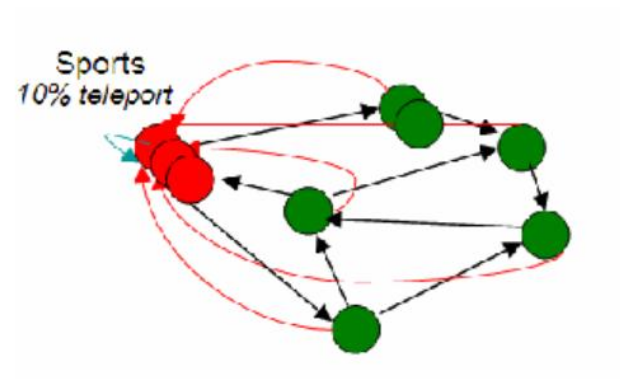
\includegraphics[scale=0.4]{GraphImportance//img/esempioslide.png}
\end{figure}
\\
Dato che l'insieme \( S \) delle pagine relative allo sport non è vuoto, ne consegue che esiste un insieme non vuoto di pagine web \( Y \supseteq S \) sul quale la random walk ha una distribuzione stazionaria; indichiamo questa distribuzione di PageRank specifica per lo sport con \( \pi_S \). Per le pagine web che non appartengono a \( Y \), assegniamo un valore di PageRank pari a zero. Chiamiamo \( \pi_S \) il PageRank specifico per l'argomento "sport".

\paragraph{Utilizzo topic-specific PageRank} Il PageRank specifico diventa una misura di similarity, e puó trovare diverse applicazioni come ad esempio:
\begin{quote}
    Qual é la probabilitá di arrivare al nodo B, partendo dal nodo A? 
\end{quote}
Per rispondere a questa domanda potremmo passare per i nodi piú rilevanti per il nodo A grazie al PageRank specifico. L'esempio piú frequente é quello del movie recommendation: sapendo che ti é piaciuto un film (nodo) consigliami un altro (film che fanno parte di un subset $S$ connesso al nodo attuale).
\newpage
\subsubsection*{Particle Filtering Approach}
L'approccio a filtraggio a particelle (\textit{Particle Filtering}) è una tecnica di campionamento stocastico utilizzata per stimare distribuzioni di probabilità in sistemi dinamici. Applicato ai grafi, esso consente di approssimare distribuzioni di PageRank o cammini di navigazione in modo efficiente, anche quando la dimensione del grafo è elevata o quando si desidera un PageRank specifico per un argomento.

Sia \( G = (V, E) \) un grafo diretto, dove \( V \) è l'insieme dei nodi (pagine) e \( E \) è l'insieme degli archi (link).

L'algoritmo si basa sui seguenti passaggi principali:

\begin{itemize}
    \item \textbf{Inizializzazione}: vengono generate \( N \) particelle, ognuna rappresenta una posizione iniziale su un nodo \( v \in V \), tipicamente campionato da una distribuzione iniziale \( p_0(v) \), ad esempio una distribuzione uniforme o una distribuzione concentrata su un sottoinsieme \( S \subseteq V \) (per topic-specific PageRank).
    
    \item \textbf{Propagazione}: ad ogni passo \( t \), ogni particella si sposta su un vicino del nodo corrente secondo la matrice di transizione \( P \), definita da:
    \[
        P_{ij} = \beta \cdot \frac{1}{\deg^+(v_i)} + (1 - \beta) \cdot \frac{1}{|V|}
    \]
    dove \( \deg^+(v_i) \) è il numero di link uscenti dal nodo \( v_i \), e \( \beta \in [0,1] \) è il parametro di damping.
    
    \item \textbf{Resampling (opzionale)}: per evitare la degenerazione (ossia la concentrazione eccessiva delle particelle in pochi nodi), si può applicare un'operazione di \textit{resampling}, dove le particelle vengono ricampionate in base alla loro importanza o peso.
    
    \item \textbf{Stima}: dopo un numero sufficiente di iterazioni \( T \), la distribuzione delle particelle sui nodi del grafo fornisce una stima empirica della distribuzione stazionaria desiderata:
    \[
        \hat{\pi}(v) = \frac{\# \text{ particelle in } v}{N}
    \]
\end{itemize}

Questo metodo è particolarmente utile per calcolare il PageRank su grandi grafi o per versioni personalizzate e dinamiche del PageRank (es. topic-specific, temporal, personalized), dove i metodi tradizionali di moltiplicazione matriciale risulterebbero troppo costosi. [fonte GPT]

\paragraph{Aggiunta slide} Nelle slide viene evidenziato il fatto che si tratti di un metodo che approssima l'importanza dei nodi di un grafo simulando il moto di particelle. Archi differenti hanno rilevanza diversa. Le particelle si posizionano in un nodo qualsiasi all'istante iniziale poi si diffondono seguendo la \textbf{edge importance}. La dissipazione assicura che le particelle eventualmente finiscano su nodi importanti. 